\section{Design Pattern - Memento}
\label{sec:memento}

\hspace{5mm} O \textbf{Memento} é um design pattern que permite ir guardando várias versões do estado ao longo do tempo, permitindo assim voltar a um estado anterior.

\begin{figure}[H]
    \centering
    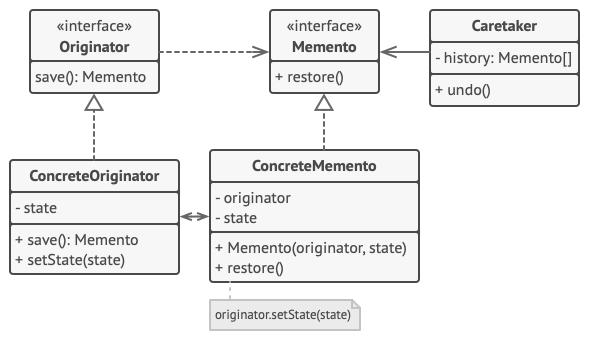
\includegraphics[scale=0.55]{images/generic_memento_class_diagram.png}
    \caption{Arquitetura genérica do design pattern Memento.}
    \label{fig:diagrama-classes-memento}
\end{figure}

\begin{figure}[H]
    \centering
    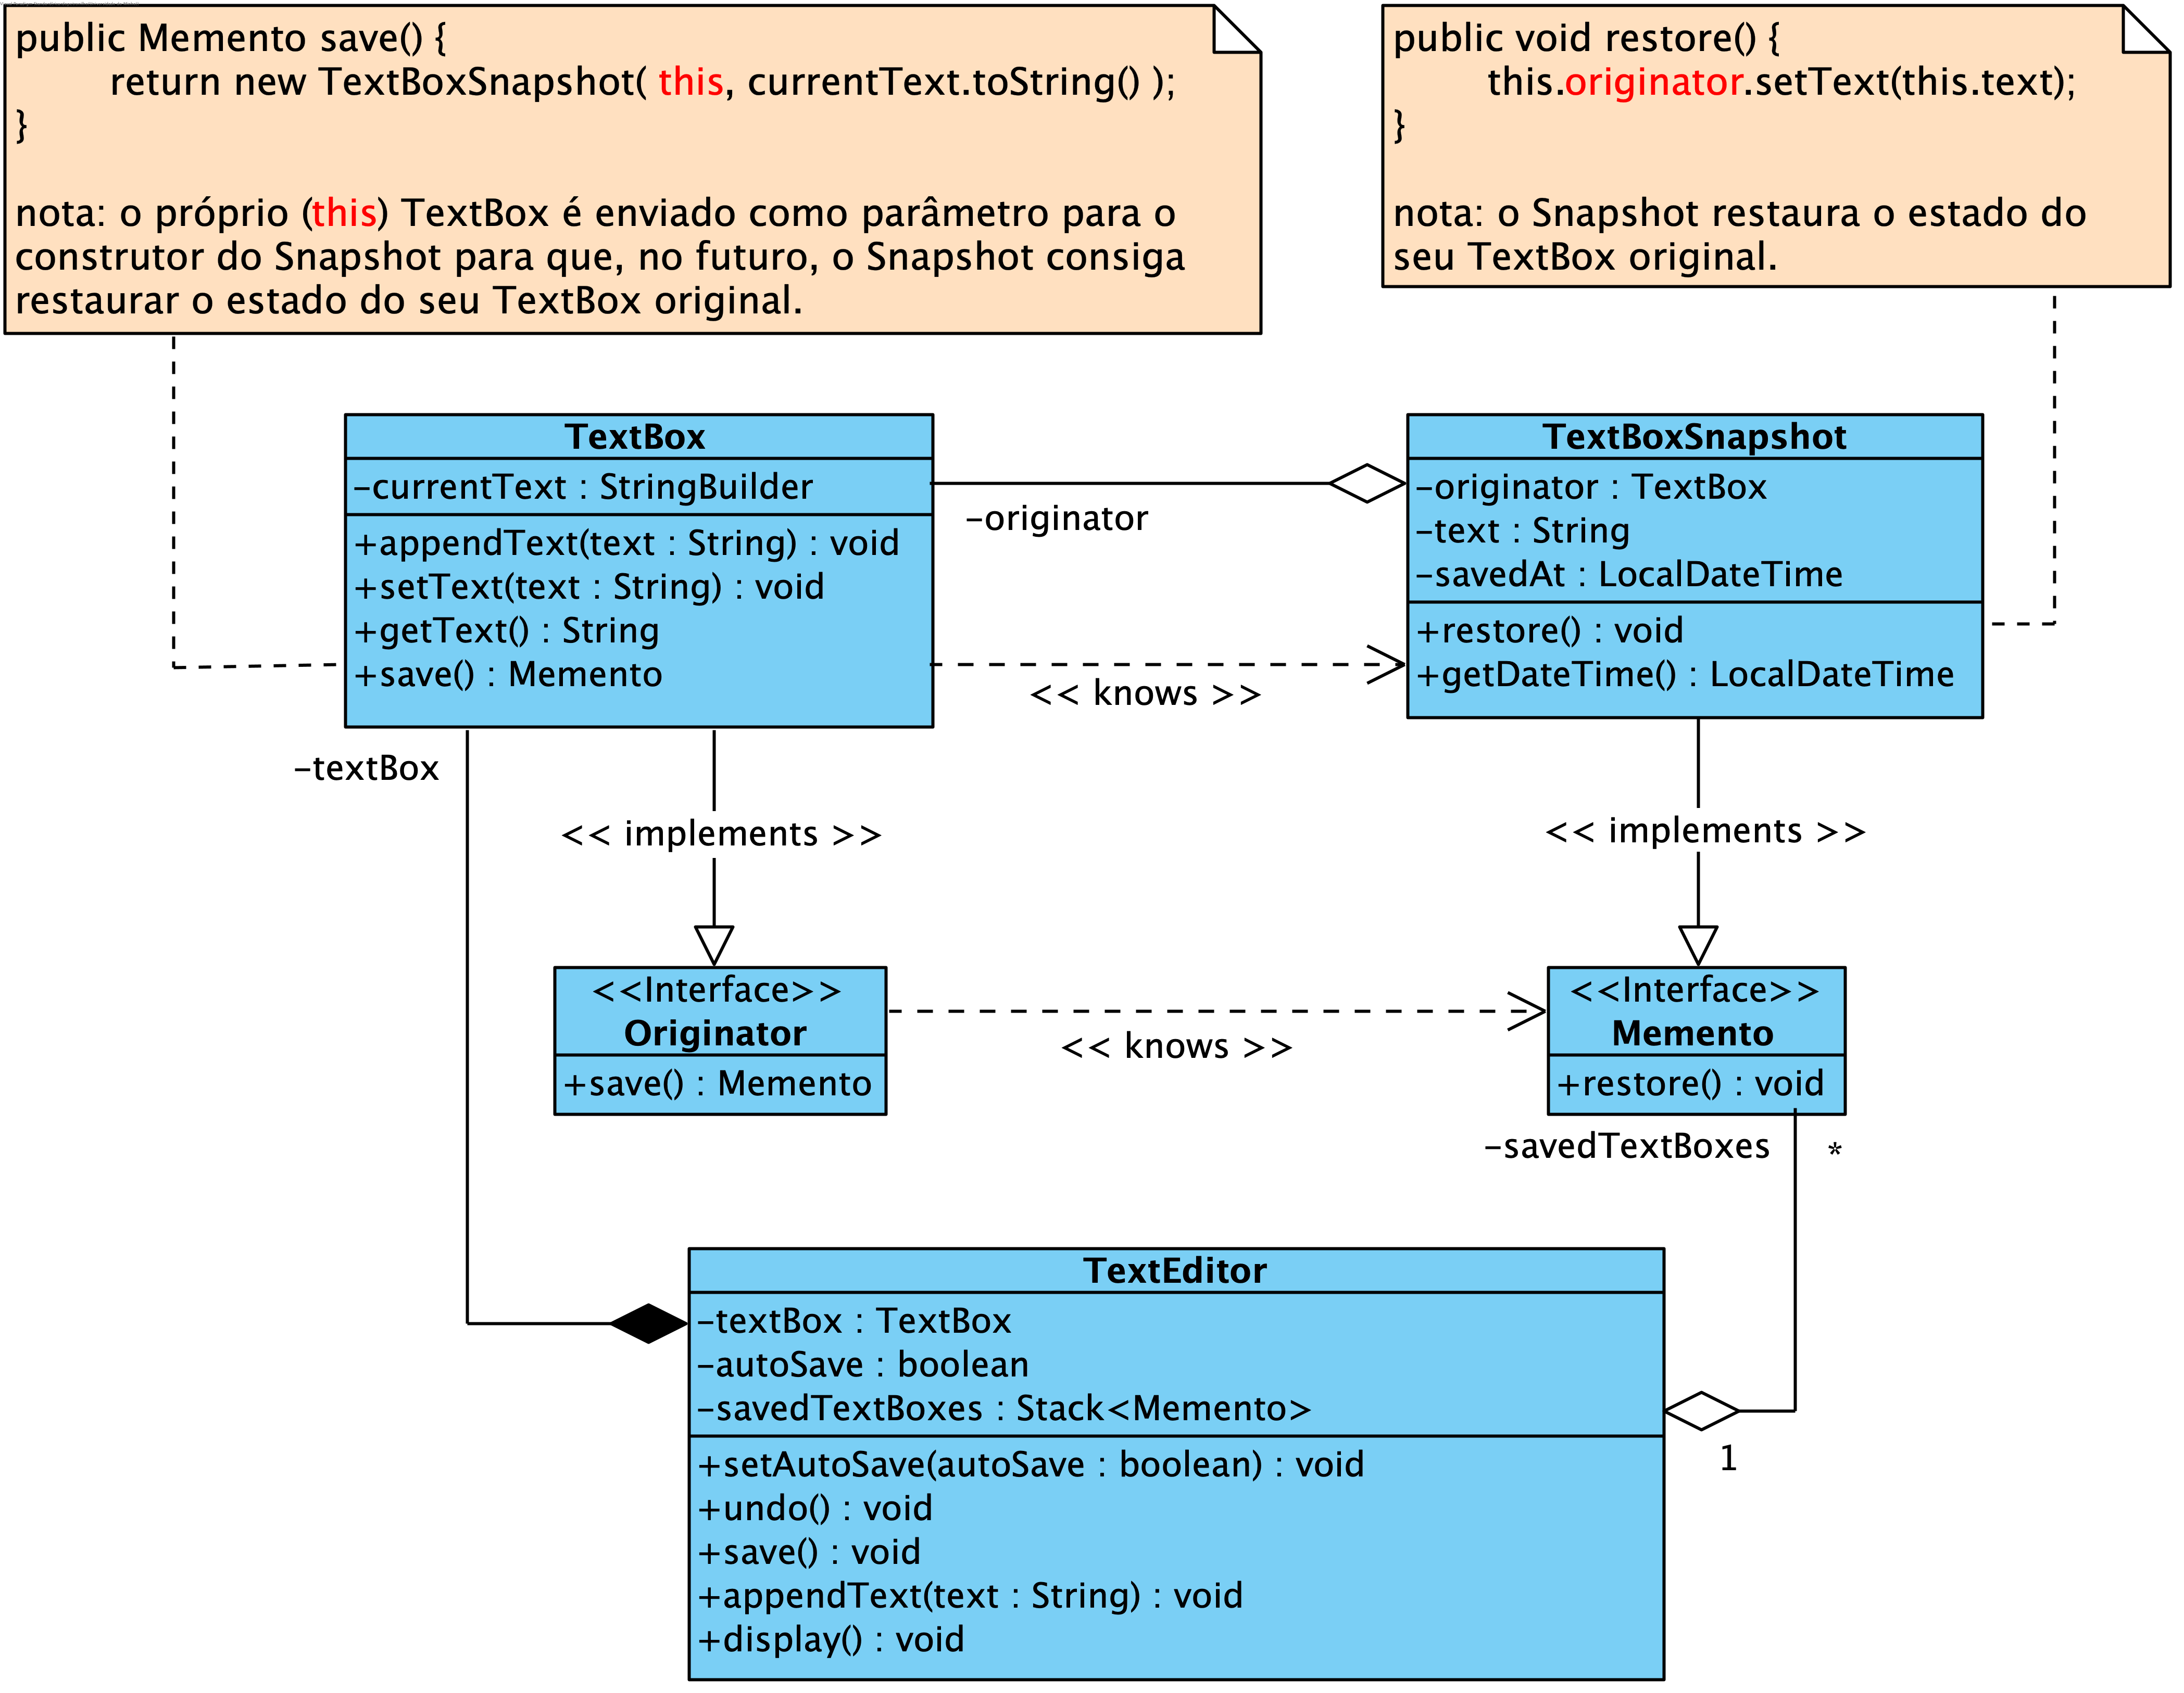
\includegraphics[scale=0.8]{images/memento_class_diagram.png}
    \caption{Arquitectura de um editor de texto usando o design pattern Memento.}
    \label{fig:diagrama-classes-memento}
\end{figure}

\hspace{2mm} Na figura acima está representada a arquitectura deste \textit{design pattern} com um pequeno exemplo implementado. 

\hspace{2mm} Quando se quer gravar os novos estados gerados num \textbf{TextBox} existem duas formas de o fazer:
\begin{itemize}
    \item invocando o método \textbf{save()} no \textbf{TextEditor} que cria um novo snapshot do estado atual e guarda-o na stack.
    \newline
    
    \item outra forma opcional, utilizada neste exemplo em específico, é colocar a variável \textit{autoSave} a \textit{true}, assim sempre que é feita uma alteração ao estado é criado automaticamente um snapshot e adicionado à stack através da operação \textit{push()}.
    \newline
    
\end{itemize}

\hspace{2mm} No TextEditor sempre que se quiser que os seus componentes voltem a um estado anterior basta invocar o método \textbf{undo()}, este método vai interagir com a variável \textit{savedTextBoxes} que é uma \textit{Stack} de \textbf{Memento} (instância de \textbf{TextBoxSnapshot}), ou seja, sempre que se pretende fazer o \textit{undo()} será realizado um \textit{pop()}, garantindo que se vai buscar o estado exactamente anterior ao momento da invocação. Depois de se obter o estado exactamente anterior ao estado actual é realizado o \textit{restore()} à variável do tipo \textbf{Memento} que irá reverter o estado actual do TextBox associado à mesma.

\hspace{2mm} Existem duas alternativas arquitecturais possíveis para reverter o estado do TextBox. 
\newline

\begin{itemize}
    
    \item 1ª alternativa: o próprio TextBox tem o método - \textbf{restore(TextBoxSnapshot s)} - que recebendo \textbf{qualquer} snapshot reverte o seu estado para o indicado no snapshot.
    Note-se que esta alternativa pode ter um \textbf{problema de integridade} uma vez que torna possível um TextBox reverter para um estado de \textbf{outro} TextBox, o que à partida apenas devia ser possível reverter para um estado que anteriormente foi do \textbf{próprio}. 
    \newline
    
    \item 2ª alternativa: no momento que o TextBox cria uma \textbf{TextBoxSnapshot} é enviado como parâmetro para este último o TextBox que o criou - \textbf{originator} - desta forma o método - \textbf{restore()} - encontra-se no TextBoxSnapshot, tornando-se impossível que um TextBox reverta o seu estado para outro que não seja anteriormente do próprio.
    \newline
    
\end{itemize}

\hspace{2mm} A arquitetura apresentada neste documento segue a 2ª alternativa. Note-se que apesar da 1ª alternativa manifestar um problema de integridade, pode ser usada propositadamente, o contexto do problema que se pretende resolver é que motiva os dois tipos de implementação.

\hspace{2mm} Neste momento poderá estar a questionar-se sobre o motivo da criação de uma nova classe TextBoxSnapshot para guardar uma cópia do estado de um TextBox. A forma mais simples de o fazer seria, por exemplo, criar um método - \textbf{TextBox clone()} - que devolve um novo TextBox exatamente igual em valor. No entanto, dessa forma, o novo TextBox clonado não só guarda uma cópia do valor como também o \textbf{comportamento} e isso pode \textbf{não ser seguro}. Desta forma ao criar uma nova classe TextBoxSnapshot apenas se copia o estado e respetivamente os métodos get() para aceder ao estado, no entanto o \textbf{comportamento está propositadamente omisso}.

\hspace{2mm} No anexo \ref{anexo:memento} pode-se visualizar a implementação do diagrama de classes apresentado em cima. 